\def\GelfandPackingCaption{вписываем}
\begin{center}
\begin{minipage}[t]{.46\linewidth}\vspace{0pt}\centering
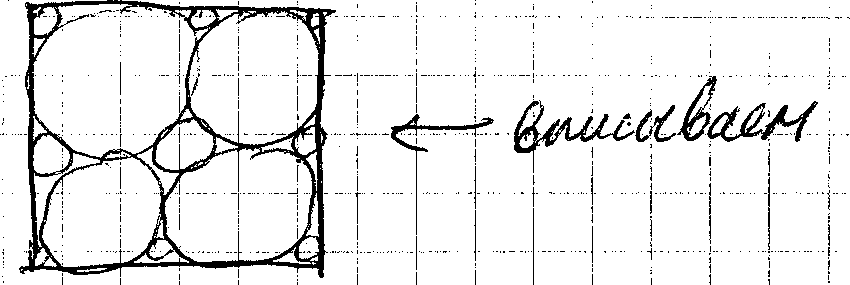
\includegraphics[width=\linewidth]{figures/gelfand-0153-p001410-circle-packing-original-r2.png}\par\smallskip
{\footnotesize Оригинал рукописного рисунка: \texttt{GELFAND-P001410}}
\end{minipage}\hfill
\begin{minipage}[t]{.50\linewidth}\vspace{0pt}\centering
{\footnotesize Частичное воссоздание видимых штрихов}\par\smallskip
\resizebox{\linewidth}{!}{% Hand-drawn contours; these coordinates do not specify exact tangencies or radii.
\begin{tikzpicture}[x=.7cm,y=.7cm]
\draw (0,0) rectangle (3,2.7);
\draw (.75,1.07) .. controls (-.05,1.16) and (-.06,2.58) .. (.7,2.64)
 .. controls (1.55,2.92) and (1.64,1.72) .. (1.43,1.37)
 .. controls (1.31,1.19) and (1.06,1.06) .. (.75,1.07);
\draw (1.5,1.43) .. controls (1.36,2.1) and (1.85,2.91) .. (2.4,2.65)
 .. controls (3.12,2.66) and (3.14,1.55) .. (2.51,1.28)
 .. controls (2.03,1.15) and (1.65,1.23) .. (1.5,1.43);
\draw (.21,.17) .. controls (.12,.76) and (.51,1.24) .. (.92,1.06)
 .. controls (1.52,.85) and (1.51,.29) .. (1.12,.08)
 .. controls (.69,-.13) and (.27,-.02) .. (.21,.17);
\draw (1.43,.31) .. controls (1.38,.73) and (1.84,1.19) .. (2.35,1.18)
 .. controls (3.14,1.34) and (3.14,.44) .. (2.79,.17)
 .. controls (2.29,-.07) and (1.56,-.07) .. (1.43,.31);
\draw (.02,2.42) .. controls (.3,2.39) and (.41,2.69) .. (.12,2.67)--cycle;
\draw (1.45,2.7) .. controls (1.66,2.32) and (1.86,2.7) .. (1.7,2.7);
\draw (2.82,2.63) .. controls (3.08,2.48) and (3.02,2.65) .. (3,2.7);
\draw (.05,.89) .. controls (.36,.75) and (.46,1.11) .. (.05,1.26)--cycle;
\draw (1.3,1.12) .. controls (1.01,.85) and (1.69,.81) .. (1.78,1.21)
 .. controls (1.65,1.44) and (1.53,1.49) .. (1.3,1.12);
\draw (2.8,1.34) .. controls (3.2,.86) and (2.71,.94) .. (2.8,1.34);
\draw (.02,.17) .. controls (.34,.04) and (.14,.3) .. (.02,.17);
\draw (1.18,.06) .. controls (1.42,.38) and (1.63,.02) .. (1.18,.06);
\draw (2.84,.04) .. controls (2.64,.24) and (3.03,.32) .. (3,.04)--cycle;
\draw[->] (4.05,1.28)--(3.43,1.23);
\node[right] at (4.05,1.28) {\GelfandPackingCaption};
\end{tikzpicture}
}
\end{minipage}
\end{center}
\noindent{\small\textit{Видимые контуры воссозданы приближённо. Точные касания, размеры окружностей и принадлежность мелких граничных дуг не установлены; количественная упаковка не задана.}}
